%\title{emnlp 2017 instructions}
% File emnlp2017.tex
%

\documentclass[11pt,letterpaper]{article}
\usepackage{emnlp2017}
\usepackage{times}
\usepackage{latexsym}
\usepackage{graphicx}

% Uncomment this line for the final submission:
%\emnlpfinalcopy

%  Enter the EMNLP Paper ID here:
\def\emnlppaperid{***}

% To expand the titlebox for more authors, uncomment
% below and set accordingly.
% \addtolength\titlebox{.5in}    

\newcommand\BibTeX{B{\sc ib}\TeX}


\title{Including lexical morphosyntactic information\\in a neural PoS tagging architecture}

% Author information can be set in various styles:
% For several authors from the same institution:
% \author{Author 1 \and ... \and Author n \\
%         Address line \\ ... \\ Address line}
% if the names do not fit well on one line use
%         Author 1 \\ {\bf Author 2} \\ ... \\ {\bf Author n} \\
% For authors from different institutions:
% \author{Author 1 \\ Address line \\  ... \\ Address line
%         \And  ... \And
%         Author n \\ Address line \\ ... \\ Address line}
% To start a seperate ``row'' of authors use \AND, as in
% \author{Author 1 \\ Address line \\  ... \\ Address line
%         \AND
%         Author 2 \\ Address line \\ ... \\ Address line \And
%         Author 3 \\ Address line \\ ... \\ Address line}
% If the title and author information does not fit in the area allocated,
% place \setlength\titlebox{<new height>} right after
% at the top, where <new height> can be something larger than 2.25in
%\author{Siddharth Patwardhan \and Preethi Raghavan \\
%  {\tt publication@emnlp2017.net}}
\author{Anonymous submission}

\date{}

\begin{document}

\maketitle

\begin{abstract}
  Abstract
\end{abstract}


\section{Introduction}

Part-of-speech tagging is now a classic task in natural language processing, for which many systems have been developed
or adapted for a large variety of languages. Its aim is to associate each ``word'' with a morphosyntactic tag, whose
granularity can range from a simple morphosyntactic category, or part-of-speech (hereafter PoS), to finer categories
enriched with morphological features (gender, number, case, tense, mood, etc.).

The use of machine learning algorithms trained on manually annotated corpora has long become the standard way to develop
PoS taggers. A large variety of algorithms have been used, such as (in approximative chronological order) bigram and
trigram hidden Markov models \cite{merialdo94,brants96,brants00}, decision trees \cite{schmid94,magerman95}, maximum
entropy Markov models (MEMMs) \cite{ratnaparkhi96} and Conditional Random Fields (CRFs)
\cite{lafferty01,constant12}. Recently, neural approaches have reached very competitive accuracy levels, improving over
the state of the art in an number of settings \cite{plank16}.

As a complement to the annotated corpora used to train such systems, external lexical information has been shown to be
valuable sources of information. First, morphosyntactic lexicons, which provide a large inventory of (word,~PoS)
pairs. Such lexical information can be used in the form of constraints at tagging time \cite{kim99,hajic00tagging} or
during the training process as additional features combined with standard features extracted from the training corpus
\cite{chrupala08,goldberg09,denis12}.

Second, lexical information encoded in the form of vector representations, known as word embeddings, have
emerged more recently \cite{bengio03,collobert08,chrupala13,ling15,ballesteros15,muller15}. Such representations, which
are generally extracted from large amounts of raw text, have proved very useful for numerous tasks including PoS
tagging, in particular when used in recurrent neural networks (RNNs) and more specifically in mono- or bi-directional,
word-level and/or character-level long short-term memory networks (LSTMs)
\cite{hochreiter97,ling15,ballesteros15,plank16}.

However, the inclusion of lexical information from morphosyntactic lexicons into neural PoS tagging architecture, as a
replacement or complement to pre-computed word embeddings, remains to be investigated. In this paper, we describe how
such an inclusion can be achieved and show, based on experiments on all corpora from the Universal Dependencies
repository (version 1.3), that it leads to significant improvements over \citeauthor{plank16}'s (\citeyear{plank16}).
state-of-the-art results.

\section{Baseline bi-LSTM tagger}

As shown by \citet{plank16}, state-of-the-art performance can be achieved using a bi-LSTM architecture fed with word
representations. Optimal performance is achieved representing words using the concatenation of (i) a word vector
$\vec{w}$ built using a word embedding layer, and (ii) a representation $\vec{c}$ of the word's characters built using a
character-level bi-LSTM, which is trained jointly with the word-level layers. Further improvements can be obtained on
most but not all languages by initialising the word embedding layer with pre-computed word embeddings. We refer to
\citet{plank16} for further details.\footnote{In our work, we did not use \citeauthor{plank16}'s (\citeyear{plank16})
  idea of a secondary task aimed at predicting the frequency class of each word. Integrating this secondary task in
  their bi-LSTM architecture, the authors obtain better OOV scores but virtually identical overall scores when averaged
  over all tested languages/corpora. We therefore decided to stick to the standard one-task architecture. }

\section{Integrating lexical morphosyntactic information}

\begin{figure*}
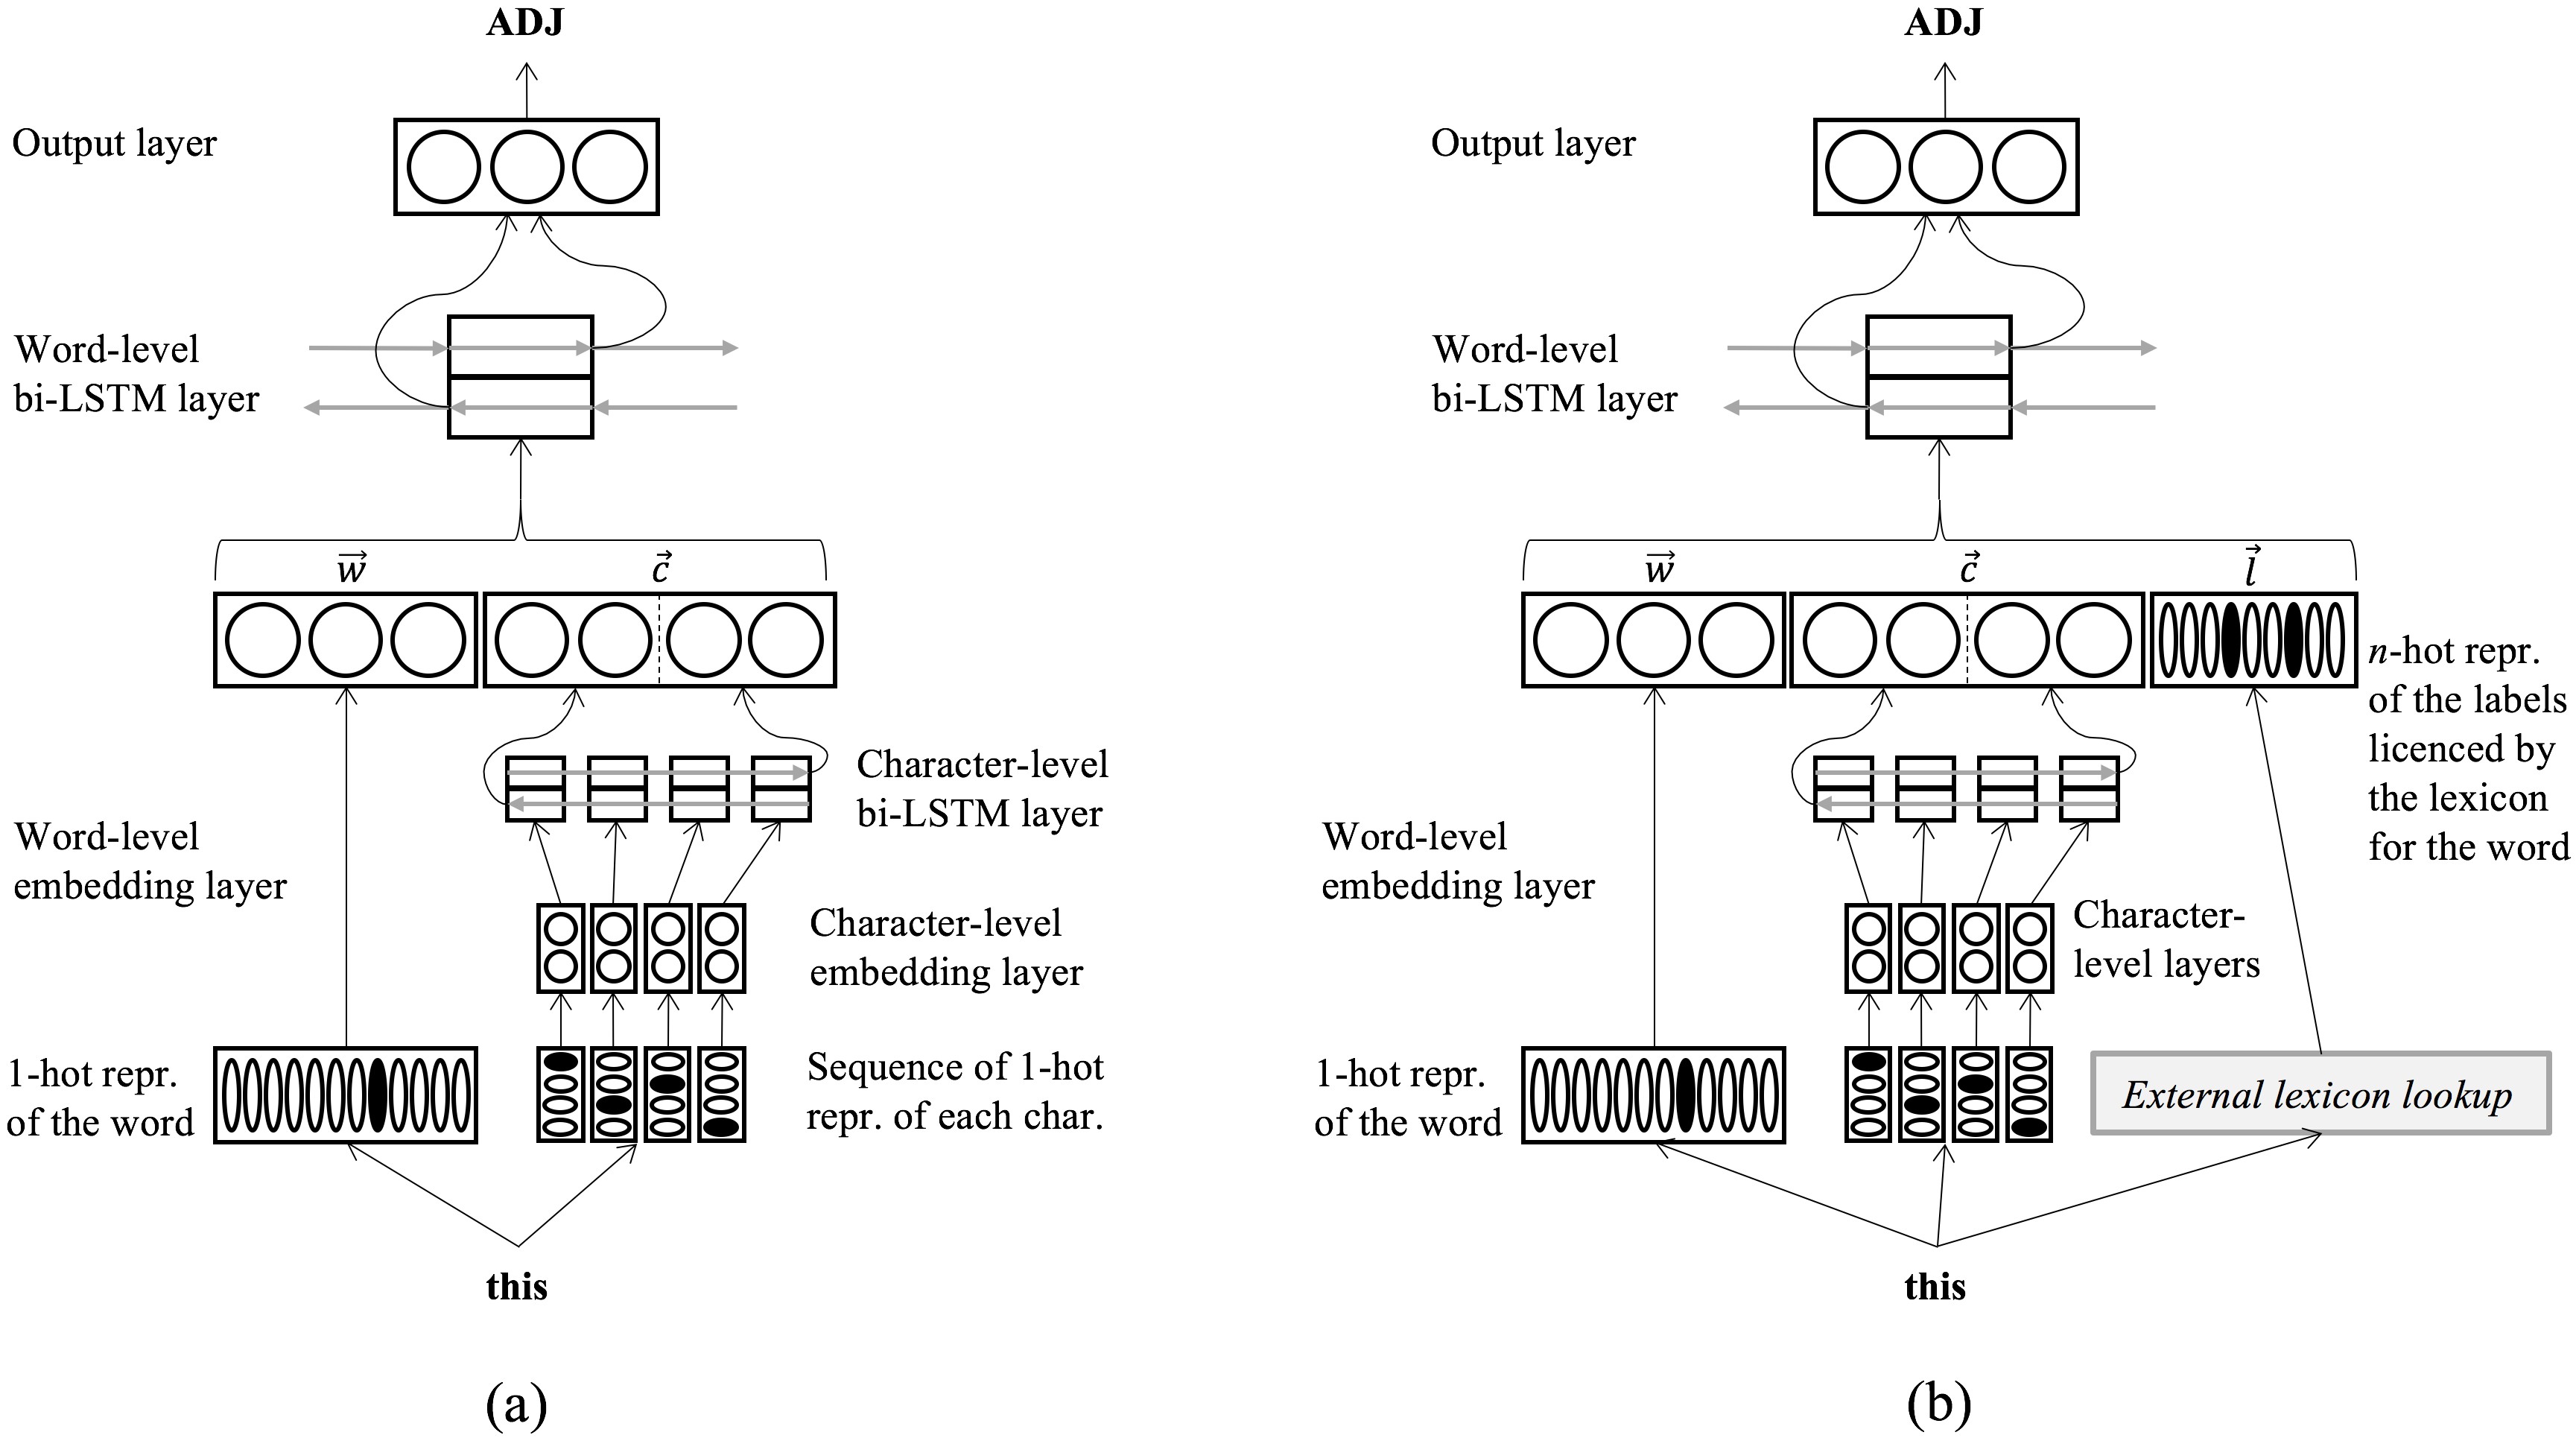
\includegraphics[width=\linewidth]{emnlp17schema}
\caption{Schematic representation of the architecture of (a)~\citeauthor{plank16}'s (\citeyear{plank16}) bi-LSTM tagger,
and (b)~our extension thereof for integrating external morphosyntactic lexical information. Each of these two schemas
represent concern a single word. Connections of the word-level LSTM cells to their counterparts for the preceeding and
following word are represented with grey arrows.}\label{fig:schema}
\end{figure*}

\section{Experimental setup}

We use as a baseline the state-of-the-art bi-LSTM PoS tagger \texttt{bilty}, a freely
available\footnote{\url{https://github.com/bplank/bilstm-aux}} and ``significantly refactored version of the code
originally used in'' \cite{plank16}. We use its best-performing configuration, which consists in using both word-level
and character-level embeddings and 3 stacked bi-LSTM layers.

\section{Results and discussion}


%\section*{Acknowledgments}



\bibliography{emnlp17}
\bibliographystyle{emnlp_natbib}

\end{document}
